% Author: Izaak Neutelings (October 2021)
% Inspiration
%   "Very special relativity - An illustrated guide", Sander Bais (2007)
\documentclass[border=3pt,tikz]{standalone}
\usepackage{tikz}
\usepackage{amsmath} % for \text
\usepackage{etoolbox} % ifthen
\usepackage[outline]{contour} % glow around text
\usetikzlibrary{decorations.markings,decorations.pathmorphing}
\usetikzlibrary{angles,quotes} % for pic (angle labels)
\usetikzlibrary{arrows.meta} % for arrow size
\usepackage{xfp} % higher precision (16 digits?)
\contourlength{1.1pt}

\newcommand{\calI}{\mathscr{I}} %\mathcal
\tikzset{>=latex} % for LaTeX arrow head
\colorlet{myred}{red!80!black}
\colorlet{myblue}{blue!80!black}
\colorlet{mygreen}{green!80!black}
\colorlet{mydarkred}{red!55!black}
\colorlet{mydarkblue}{blue!50!black}
%\colorlet{mylightblue}{blue!60!black!30}
\colorlet{mypurple}{blue!40!red!80!black}
\colorlet{mydarkgreen}{green!50!black}
\colorlet{mydarkpurple}{blue!40!red!50!black}
%\colorlet{mylightpurple}{mydarkpurple!80!red!6}
\colorlet{myorange}{orange!40!yellow!95!black}
\colorlet{mydarkorange}{orange!40!yellow!85!black}
\tikzstyle{world line}=[myblue!60,line width=0.4]
\tikzstyle{world line t}=[mypurple!60,line width=0.4]
\tikzstyle{world line'}=[mydarkred!60,line width=0.4]
\tikzstyle{mysmallarr}=[-{Latex[length=3,width=2]},thin]
\tikzstyle{mydashed}=[dash pattern=on 3 off 3]
\tikzstyle{vector}=[->,line width=1,line cap=round]
\tikzstyle{vector'}=[vector,shorten >=1.2]
%\tikzstyle{measure}=[{Latex[length=3,width=2]}-{Latex[length=3,width=2]},thin]
\tikzstyle{particle}=[mygreen,line width=0.9]
\tikzstyle{photon}=[-{Latex[length=5,width=4]},myorange,line width=0.8,decorate,
                    decoration={snake,amplitude=1.0,segment length=5,post length=5}]

\def\tick#1#2{\draw[thick] (#1) ++ (#2:0.06) --++ (#2-180:0.12)}
\def\tickp#1#2{\draw[thick,mydarkred] (#1) ++ (#2:0.06) --++ (#2-180:0.12)}
\def\Nsamples{40} % number samples in plot

\begin{document}


% LORENTZ FACTOR
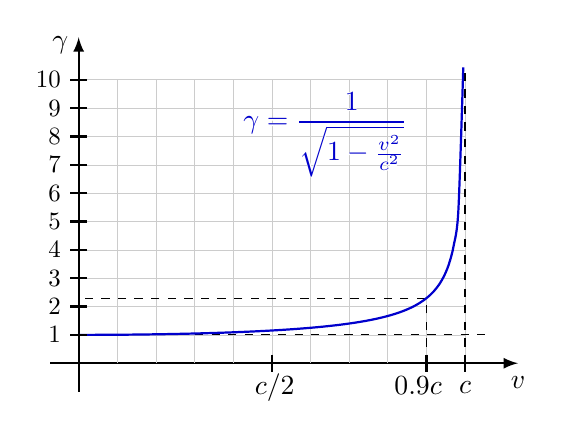
\begin{tikzpicture}[scale=1.8]
  \message{Lorentz factor^^J}
  
  \def\xmax{2.9}
  \def\ymax{2.1}
  \def\A{0.2} % amplitude / y scale
  \pgfmathsetmacro\c{0.94*\xmax} % speed of light
  \coordinate (O) at (0,0);
  
  % AXES
  \draw[->,thick] (-0.2,0) -- (\xmax+0.2,0) node[below=1] {$v$};
  \draw[->,thick] (0,-0.2) -- (0,\ymax+0.2) node[below=3,left=0] {$\gamma$};
  
  % GRID
  \foreach \i in {1,...,10}{
    \draw[black!20,very thin] (0,\i*\A) --++ (\c,0);
    \draw[black!20,very thin] (\i*\c/10,0) --++ (0,10*\A);
  }
  
  % PLOT
  \draw[dashed] (0,\A) --++ (\xmax,0);
  \draw[dashed] (\c,0) --++ (0,\ymax);
  \draw[dashed] (0.9*\c,0) |- (0,{\A/sqrt(1-0.9^2)});
  \draw[myblue,thick,samples=2*\Nsamples,smooth,variable=\v,domain=0:{\c*sqrt(1-(\A/\ymax)^2)}]
    plot(\v,\fpeval{\A/sqrt(1-(\v/\c)^2)});
  \node[myblue,below=1] at (0.6*\xmax,10*\A)
    {\contour{white}{$\gamma=\dfrac{1}{\sqrt{1-\frac{v^2}{c^2}}}$}};
  
  % TICKS
  \tick{\c/2,0}{90} node[right=1,below=-3] {$c/2$};
  \tick{0.9*\c,0}{90} node[left=3,below=-2] {$0.9c$};
  \tick{\c,0}{90} node[below=0] {$c$};
  \foreach \i in {1,...,10}{
    \tick{0,\i*\A}{0} node[left,scale=0.9] {$\i$};
  }
  
\end{tikzpicture}


\end{document}